% $Id: Grid_desc.tex,v 1.33 2007/08/24 16:09:00 murphysj Exp $
%
% Earth System Modeling Framework
% Copyright 2002-2008, University Corporation for Atmospheric Research, 
% Massachusetts Institute of Technology, Geophysical Fluid Dynamics 
% Laboratory, University of Michigan, National Centers for Environmental 
% Prediction, Los Alamos National Laboratory, Argonne National Laboratory, 
% NASA Goddard Space Flight Center.
% Licensed under the University of Illinois-NCSA License.

The ESMF Grid class is used to describe the geometry and discretization
of logically rectangular physical grids.  It also contains the
description of the grid's underlying topology and the decomposition
of the physical grid across the available computational resources.
The most frequent use of the Grid class is to describe physical grids
in user code so that sufficient information is available to perform ESMF
methods such as regridding.  

In the current release (v3.0.3)
the functionality in this class is partially implemented.  
Multi-tile grids are not supported, and edge connectivities 
are not implemented and default to aperiodic.  Only irregular 
distributions can be defined.  Specific interfaces for regular
and arbitrary distributions have not been implemented, though
regular distributions can be defined as a special case of 
irregular distributions.  Also, each coordinate array in a 
grid has the full rank of the grid itself (i.e., the grid
is assumed to be curvilinear).  Other constraints of the current
implementation are noted in the usage section and in the API
descriptions.

\begin{center}
\begin{tabular}{|p{6in}|}
\hline
\vspace{.01in}
{\bf Key Features} \\[.01in]
Representation of grids formed by logically rectangular regions,
including uniform and rectilinear grids (e.g. lat-lon grids),
curvilinear grids (e.g. displaced pole grids), and grids formed
by connected logically rectangular regions (e.g. cubed sphere grids)
[CONNECTED REGIONS ARE NOT YET SUPPORTED].\\
Support for 1D, 2D, 3D, and higher dimension grids.\\ 
Distribution of grids across computational resources for parallel
operations - users set which grid dimensions are distributed.\\
Grids can be created already distributed, so that no single
resource needs global information during the creation process.\\
Options to define periodicity and other edge connectivities either 
explicitly or implicitly via shape shortcuts [EDGE CONNECTIVITIES
CURRENTLY DEFAULT TO APERIODIC BOUNDS].\\ 
Options for users to define grid coordinates themselves or call
prefabricated coordinate generation routines for standard grids
[NO GENERATION ROUTINES YET].\\
Options for incremental construction of grids.\\
Options for using a set of pre-defined stagger locations or for setting
custom stagger locations.\\ [.03in] \hline
\end{tabular}
\end{center}

\subsubsection{Grid Representation in ESMF}

ESMF Grids are based on the concepts described in {\it A Standard
Description of Grids Used in Earth System Models} [Balaji 2006].  In this document
Balaji introduces the mosaic concept as a means of describing
a wide variety of Earth system model grids.  A {\bf mosaic} is
composed of grid tiles connected at their edges.  Mosaic grids
includes simple, single tile grids as a special case.  

The ESMF Grid class is a representation of a mosaic grid.  Each ESMF
Grid is constructed of one or more logically rectangular {\bf Tiles}.
A Tile will usually have some physical significance (e.g. the region
of the world covered by one face of a cubed sphere grid).

The piece of a Tile that resides on one DE (for simple cases, a DE
can be thought of as a processor - see section on the DELayout)
is called a {\bf LocalTile}.  For example, the six faces of a cubed
sphere grid are each Tiles, and each Tile can be divided into many
LocalTiles.  

Every ESMF Grid contains a DistGrid object, which defines the Grid's
index space, topology, distribution, and connectivities.  It enables
the user to define the complex edge relationships of tripole and other
grids.  The DistGrid can be created explicitly and passed into a Grid
creation routine, or it can be created implicitly if the user takes
a Grid creation shortcut.  Options for grid creation are described in 
more detail in section \ref{sec:gridcreateoptions}.

\subsubsection{Supported Grids}

The range of supported grids in ESMF can be defined by:
\begin{itemize}
\item Types of topologies and shapes supported.  ESMF supports one or
more logically rectangular grid Tiles with connectivities specified
between cells.  For more details see section \ref{sec:ShapeShortcut}.
\item Types of distributions supported.  ESMF supports  regular,
irregular, or arbitrary distributions of data.  Note that arbitrary
distributions have not been implemented as of v3.0.3.
For more details see section \ref{sec:desc:dist}.
\item Types of coordinates supported.  ESMF supports uniform, rectilinear,
and curvilinear coordinates.  For more details see section \ref{sec:coordspec}.
\end{itemize}

\subsubsection{Grid Topologies and Periodicity}
\label{sec:ShapeShortcut}
ESMF has shortcuts for the creation of standard Grid topologies 
or {\bf shapes} up to 3D.  In many cases, these enable the user to
bypass the step of creating a DistGrid before creating the Grid.  The basic call is 
{\tt ESMF\_GridCreateShape()}.  With this call, the user can specify for
each dimension whether there is no connection, it is periodic, it
is a pole, or it is a bipole.  The assumed connectivities for poles and
bipoles are described in section \ref{sec:opt:gridconn}.  Connectivities
are specified using the ESMF\_GridConn parameter, which has values
such as ESMF\_GRIDCONN\_PERIODIC.

The table below shows the ESMF\_GridConn settings used to create 
standard shapes in 2D using the ESMF\_GridCreateShape() call.  Two values
are specified for each dimension, one for the low end and one for 
the high end of the dimension's index values.  Note that connectivities
have not been implemented as of v3.0.3 and default to aperiodic bounds.

\medskip
\begin{tabular}{|l|c|c||c|c||}
\hline
2D Shape & {\bf connDim1(1)} & {\bf connDim1(2)}  & {\bf connDim2(1)} & {\bf connDim2(2)}  \\
\hline
{\bf Rectangle}  & NONE & NONE & NONE & NONE \\
{\bf Bipole Sphere} & POLE & POLE & PERIODIC & PERIODIC \\
{\bf Tripole Sphere} & POLE & BIPOLE & PERIODIC & PERIODIC \\
{\bf Cylinder} & NONE & NONE & PERIODIC & PERIODIC \\
{\bf Torus}  & PERIODIC & PERIODIC & PERIODIC & PERIODIC \\
\hline
\hline
\end{tabular}
\medskip

If the user's grid shape is too complex for an ESMF shortcut routine,
or involves more than three dimensions, a DistGrid can be created
to specify the shape in detail.  This DistGrid is then passed
into a Grid create call.

\subsubsection{Grid Distribution}
\label{sec:desc:dist}
ESMF Grids have several options for data distribution (also referred to
as decomposition).  The user specifies which dimensions 
are to be distributed through a coordinate dependency (coordDep)
argument.

The main distribution options are regular, irregular, and arbitrary.
A {\bf regular} distribution is one in which the same number of
contiguous grid points are assigned to each DE in the
distributed dimension.  A {\bf irregular} distribution is one in which
unequal numbers of contiguous gridpoints are assigned to each
DE in the distributed dimension.  An {\bf arbitrary} distribution is
one in which any gridpoint can be assigned to any DE.  Any of these
distribution options can be applied to any of the grid shapes (i.e.,
rectangle) or types (i.e., rectilinear).  Arbitrary distributions
have not been implemented as of v3.0.3.

Figure \ref{fig:GridDecomps} illustrates options for distribution.
\begin{figure}
\scalebox{0.9}{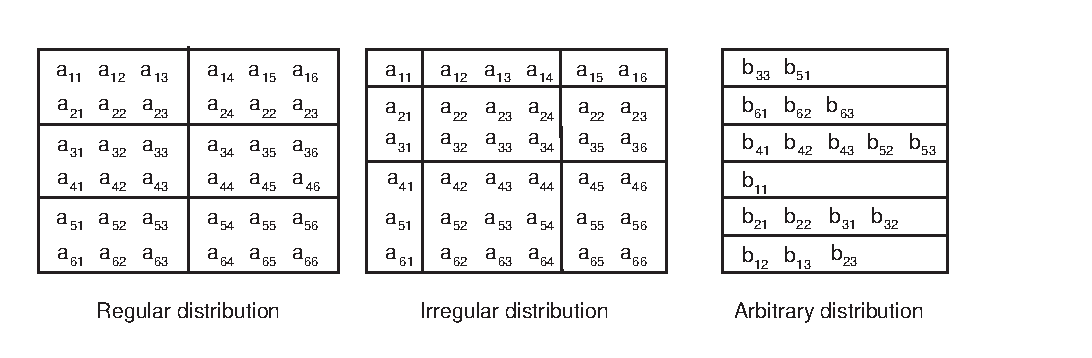
\includegraphics{GridDecomps}}
\caption{Examples of regular and irregular decomposition of
a grid {\bf a} that is 6x6, and an arbitrary decomposition of
a grid {\bf b} that is 6x3.}
\label{fig:GridDecomps}
\end{figure}

A distribution can also be specified using the DistGrid, by passing
object into a Grid create call.

\subsubsection{Grid Coordinates}
\label{sec:coordspec}
Grid Tiles can have uniform, rectilinear, or curvilinear
coordinates.  The coordinates of {\bf uniform} grids are equally spaced along
their axes, and can be fully specified by the coordinates of the two opposing points
that define the grid's physical span.  The coordinates of {\bf rectilinear} grids
are unequally spaced along their axes, and can be fully specified by giving
the spacing of grid points along each axis.  The coordinates of {\bf curvilinear 
grids} must be specified by giving the explicit set of coordinates for each
grid point.  Curvilinear grids are often uniform or rectilinear grids that 
have been warped; for example, to place a pole over a land mass so that it
does not affect the computations performed on an ocean model grid.  Figure
\ref{fig:LogRectGrids} shows examples of each type of grid.

Any of these logically rectangular grid types can be combined through edge
connections to form a mosaic.  Cubed sphere and yin-yang grids are examples
of mosaic grids.  Note that as of v3.0.3 multi-tile grids have not yet been
implemented.
 
\begin{figure}
\scalebox{0.9}{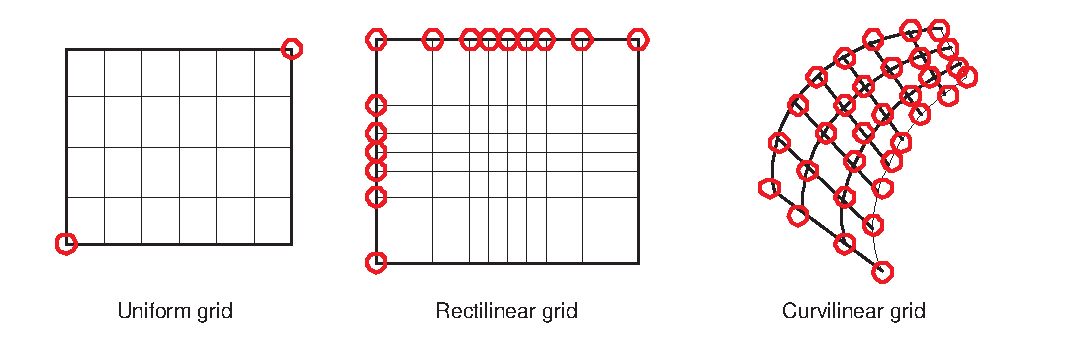
\includegraphics{LogRectGrids}}
\caption{Types of logically rectangular grid tiles.  Red circles show the
values needed to specify grid coordinates for each type.}
\label{fig:LogRectGrids}
\end{figure}

Each of these coordinate types can be set for each of the standard grid shapes
described in section \ref{sec:ShapeShortcut}.  

The table below shows how examples of common single Tile grids fall 
into this shape and coordinate taxonomy.  Note that any
of the grids in the table can have a regular or arbitrary distribution.

\medskip
\begin{tabular}{|p{.9in}|p{1.7in}|p{1.7in}|p{1.7in}|}
\hline
 & {\bf Uniform} & {\bf Rectilinear} & {\bf Curvilinear} \\ 
\hline
{\bf Sphere} & Global uniform lat-lon grid & Gaussian grid & Displaced pole grid \\
\hline
{\bf Rectangle} & Regional uniform lat-lon grid & Gaussian grid section & Polar stereographic grid section\\
\hline
\end{tabular}

\subsubsection{Coordinate Specification and Generation}

There are two ways of specifying coordinates in ESMF.  The
first way is for the user to {\bf set} the coordinates.  The second 
way is to take a shortcut and have the framework {\bf generate}
the coordinates.  

No ESMF generation routines are currently available.

See Section~\ref{sec:usage:staggerloc} for more description and examples of
setting coordinates.

\subsubsection{Staggering}

{\bf Staggering} is a finite difference technique in which the values 
of different physical quantities are placed at different locations
within a grid cell. 

The ESMF Grid class supports a variety of stagger locations, including
cell centers, corners, and edge centers.  Combinations of these are
sufficient to specify any of the Arakawa staggers.  ESMF also supports
staggering in 3D and higher dimensions.  There are shortcuts for 
standard staggers, and interfaces through which users can create custom
staggers.

As a default the ESMF Grid class provides symmetric staggering, so
that cell centers are enclosed by cell perimeter (e.g. corner) 
stagger locations. This means the coordinate arrays for stagger
locations other than the center will have an additional element of 
padding in order to enclose the cell center locations.
However, to achieve other types of staggering, the user may alter 
or eliminate this padding by using the appropriate options when adding
coordinates to a Grid. 
 
For examples and a full description of the stagger interface 
see Section~\ref{sec:usage:staggerloc}. 

\subsubsection{Options for Building Grids}
\label{sec:gridcreateoptions}

ESMF Grid objects must represent a wide range of grid types 
and use cases, some of them quite complex.  As a result, multiple
ways to build Grid objects are required.  This section describes
the stages to building Grids, the options for each stage, and 
typical calling sequences.

In ESMF there are two main stages to building Grids.  The
{\tt ESMF\_GridStatus} value stored within the Grid object reflects
the stage the Grid has attained (see Section~\ref{sec:opt:gridstatus}).
These stages are:

\begin{enumerate}

\item Create the Grid topology or shape.  At the completion of this
stage, the Grid has a specific topology and distribution, but
empty coordinate arrays.  The Grid can be used as the basis for
allocating a Field (once Grid is integrated with Field; as of 
v3.0.3, it is not).  Its {\tt ESMF\_GridStatus} parameter has 
a value of {\tt ESMF\_GRIDSTATUS\_SHAPE\_READY}.  

The options for specifying the Grid shape are:
\begin{itemize}
\item Use the {\tt ESMF\_GridCreateShape()} shortcut method to 
specify the Grid size and rank, and to select from a limited set
of edge connectivities.   
\item Create a DistGrid using the {\tt ESMF\_DistGridCreate()}
method.  This enables the user to specify connectivities in 
greater detail than using {\tt ESMF\_GridCreateShape()}.  Then
pass the DistGrid into a general {\tt ESMF\_GridCreate()} method.
\end{itemize}

\item Specify the Grid coordinates and any other information
required for regridding (this can vary depending on the particular
regridding method).  At the completion of this stage, the Grid can
be used in a regridding operation (once Grid is connected to regrid;
as of v3.0.3, it is not).  Its {\tt ESMF\_GridStatus}
has a value of {\tt ESMF\_GRIDSTATUS\_REGRID\_READY}.
\end{enumerate}

When creating the Grid shape and specifying the Grid coordinates,
the user can either specify all required information at once,
or can provide information incrementally.  The call
{\tt ESMF\_GridCreateEmpty()} builds a Grid object
container that can be filled in with subsequent calls to 
{\tt ESMF\_GridSet()} methods.  A Grid that is empty
has the {\tt ESMF\_GridStatus} value
{\tt ESMF\_GRIDSTATUS\_NOT\_READY}.

The following table summarizes possible call sequences
for building Grids.

\begin{tabular}{|l|}
\hline
{\bf Create Shape} \\
{\it From shape shortcut} \\
{\tt grid = ESMF\_GridCreateShape(...)} \\
{\it Using DistGrid with general create interface} \\
{\tt distgrid = ESMF\_DistGridCreate(...)} \\
{\tt grid = ESMF\_GridCreate(distgrid, ...)} \\
{\it Incremental} \\
{\tt grid = ESMF\_GridCreateEmpty(...)} \\
{\tt call ESMF\_GridSetShape(grid, ...)} \\ \hline
{\bf Set Coordinates} \\
{\it Set coordinates by copy or reference} \\
{\tt call ESMF\_GridSetCoord(grid, ...)} \\
{\it Retrieve ESMF Array of coordinates from Grid and set values} \\
{\tt call ESMF\_GridGetCoord(grid, ...), set values} \\
{\it Retrieve local bounds and native array from Grid and set values} \\
{\tt call ESMF\_GridGetLocalTileInfo(grid, lbound, ubound, ...)} \\
{\tt call ESMF\_GridGetLocalTileCoord(array), set values} \\ \hline
\end{tabular}
